\documentclass[8pt]{article}
 
\usepackage[margin=.8in]{geometry} 
\usepackage{amsmath,amsthm,amssymb}
\usepackage{marvosym,enumerate,color,mathrsfs,graphicx,epstopdf}
%\usepackage{enumitem}
%\setenumerate{listparindent=\parindent}
\def\cc{\color{blue}}
%\usepackage[dvipsnames]{xcolor}
\usepackage[normalem]{ulem}
\usepackage{bm}
\usepackage{mathtools}
\usepackage{mathrsfs}
\usepackage{verbatim}
\usepackage{tikz}
\usepackage[utf8]{inputenc}
\usepackage{hyperref}
\usepackage{courier}
%\usepackage{fullpage}
\usepackage{graphicx}
\usepackage{float}
\hypersetup{
	%colorlinks,
	%citecolor=black,
	%filecolor=black,
	%linkcolor=blue,
	%urlcolor=black
}

%\setlength{\oddsidemargin}{-20pt}

%\setlength{\topmargin}{-50pt}
%\setlength{\footskip}{-50pt}


%\usepackage{multirow}

%Line Numbering
\usepackage[mathlines]{lineno}
%\linenumbers
 
\newcommand{\N}{\mathbb{N}}
\newcommand{\Z}{\mathbb{Z}}
\newcommand{\R}{\mathbb{R}}
\newcommand{\C}{\mathbb{C}}
\newcommand{\Q}{\mathbb{Q}}
%\newcommand{\dell}{\partial}
\newcommand{\abs}[1]{\left\lvert{#1}\right\rvert}
\newcommand{\dx}{\mathrm{d}x}
\newcommand{\M}{\mathscr{M}}
\newcommand{\E}{\mathscr{E}}
\newcommand{\B}{\mathscr{B}}
\newcommand{\scr}[1]{\mathscr{#1}}
\newcommand{\Ns}{\mathscr{N}}
\newcommand{\nm}{\mathrel{\unlhd}}
\newcommand{\stcomp}[1]{{#1}^{\mathsf{c}}}
\newcommand{\closure}[1]{\overline{#1}}
\newcommand{\diam}{\operatorname{diam}}
\newcommand{\dist}{\operatorname{dist}}
\newcommand{\sgn}{\operatorname{sgn}}
\newcommand{\norm}[1]{\left\lVert{#1}\right\rVert}
\newcommand{\LR}[1]{\left\langle{#1}\right\rangle}

\theoremstyle{definition}
\newtheorem{theorem}{Theorem}
\newtheorem*{theorem*}{Theorem}
\newtheorem{lemma}[theorem]{Lemma}
\newtheorem{proposition}[theorem]{Proposition}
\newtheorem*{proposition*}{Proposition}
\newtheorem{definition}[theorem]{Definition}
\newtheorem*{definition*}{Definition}
\newtheorem{remark}[theorem]{Remark(s)}
\newtheorem*{remark*}{Remark(s)}
\newtheorem{corollary}[theorem]{Corollary}
\newtheorem*{corollary*}{Corollary}
\newtheorem{innerexercise}{Exercise}
\newenvironment{exercise}[1]
  {\renewcommand\theinnerexercise{#1}\innerexercise}
  {\endinnerexercise}

% Upper and lower integrals
%\def\upint{\mathchoice%
%    {\mkern13mu\overline{\vphantom{\intop}\mkern7mu}\mkern-20mu}%
%    {\mkern7mu\overline{\vphantom{\intop}\mkern7mu}\mkern-14mu}%
%    {\mkern7mu\overline{\vphantom{\intop}\mkern7mu}\mkern-14mu}%
%    {\mkern7mu\overline{\vphantom{\intop}\mkern7mu}\mkern-14mu}%
%  \int}
%\def\lowint{\mkern3mu\underline{\vphantom{\intop}\mkern7mu}\mkern-10mu\int}

\title{Numerical Analysis -- Homework 7}
\author{James Diffenderfer}
\date{\today}

%%%%%%%%%%%%%%%%%%%%%%%%%%%%%%%%%%%%%%
\begin{document}

\maketitle
%\tableofcontents

%\newpage

\begin{exercise}{1}
The modified Euler's method is 
\begin{align*}
w_0 &= \alpha \\
w_{i+1} &= w_i + \frac{h}{2} \left[ f (w_i, t_i) + f (w_i + h f (w_i, t_i), t_{i+1}) \right].
\end{align*}
Apply this method to the IVP, 
\begin{align*}
y' &= \lambda y, \ \ \lambda < 0 \\
y(0) &= 1
\end{align*}
and find the conditions on $\lambda$ and $h$ which ensure $w_{i} \to 0$ as $i \to \infty$.
\end{exercise}

\begin{proof}
From the update provided by modified Euler's method, we have that 
\begin{align*}
w_{n} &= w_{n-1} + \frac{h}{2} \left[ \lambda w_{n-1} + \lambda w_{n-1} + \lambda^2 h w_{n-1} \right] \\
&= w_{n-1} \left[ 1 + h \lambda + \frac{h^2 \lambda^2}{2} \right].
\end{align*}
Applying this formula recursively yields $$w_{n} = \alpha \left[ 1 + h \lambda + \frac{h^2 \lambda^2}{2} \right]^n.$$ Hence, it follows that $w_n \to 0$ provided that $\left| 1 + h \lambda + \frac{h^2 \lambda^2}{2} \right| < 1$. Since $\lambda < 0$ and the polynomial $1 - x + \frac{x^2}{2}$ has no real roots, it suffices to determine conditions for $h$ such that $1 + h \lambda + \frac{h^2 \lambda^2}{2} < 1$. Accordingly,
\begin{align}
1 + h \lambda + \frac{h^2 \lambda^2}{2} &< 1 \nonumber \\
\Longleftrightarrow \ \ \ \ \ \ \ \ \ \ \ \ \ \frac{h^2 \lambda^2}{2} &< - h \lambda \nonumber \\
\Longrightarrow \ \ \ \ \ \ \ \ \ \ \ \ \ \ \ \ \frac{h \lambda}{2} &> -1 \tag{Since $h > 0$ and $\lambda < 0$} \\
\Longrightarrow \ \ \ \ \ \ \ \ \ \ \ \ \ \ \ \ \ \ h &< -\frac{2}{\lambda}. \tag{Since $\lambda < 0$}
\end{align}
Since $h = 0$ results in $w_n = \alpha$ we also require that $h > 0$. Thus, we conclude that $w_n \to 0$ as $n \to \infty$ for all $h$ satisfying $0 < h < - \frac{2}{\lambda}$.
\end{proof}
\newpage



\begin{exercise}{2}
Show that the second column, $R_{k, 2}$, of Romberg integration is a composite Simpson's rule.
\end{exercise}

\begin{proof}
Define $h_k = \frac{b-a}{2^{k-1}}$ and recall that Romberg integration is defined by 
\begin{align*}
R_{k,j} = \frac{4 R_{k, j-1} - R_{k-1, j-1}}{4^{j-1} - 1},
\end{align*}
where $R_{k,1} = \frac{h_k}{2} \left[ f(a) + f(b) + 2 \sum_{i = 1}^{2^{k-1} - 1} f (a + i h_k ) \right]$. Since 
\begin{align*}
4 R_{k,1} &= 4 \cdot \frac{h_k}{2} \left[ f(a) + f(b) + 2 \sum_{i = 1}^{2^{k-1} - 1} f (a + i h_k ) \right] \\
&= h_{k} \left[ 2 f(a) + 2 f(b) + 4 \sum_{i = 1}^{2^{k-1} - 1} f (a + i h_k ) \right] \\
&= h_{k} \left[ 2 f(a) + 2 f(b) + 4 \sum_{i = 1}^{2^{k-2} - 1} f (a + (2i) h_k ) + 4 \sum_{i = 1}^{2^{k-2}} f (a + (2i + 1) h_k ) \right]
\end{align*}
and
\begin{align*}
R_{k-1,1} &= \frac{h_{k-1}}{2} \left[ f(a) + f(b) + 2 \sum_{i = 1}^{2^{k-2} - 1} f (a + i h_{k-1} ) \right] \\
&= h_{k} \left[ f(a) + f(b) + 2 \sum_{i = 1}^{2^{k-2} - 1} f (a + (2i) h_k ) \right] 
\end{align*}
it follows that
\begin{align*}
4 R_{k,1} - R_{k-1,1} = \ \ \ \ &h_{k} \left[ 2 f(a) + 2 f(b) + 4 \sum_{i = 1}^{2^{k-2} - 1} f (a + (2i) h_k ) + 4 \sum_{i = 1}^{2^{k-2}} f (a + (2i + 1) h_k ) \right] \\
- &h_{k} \left[ f(a) + f(b) + 2 \sum_{i = 1}^{2^{k-2} - 1} f (a + (2i) h_k ) \right] \\
= \ \ \ \ &h_{k} \left[ f(a) + f(b) + 2 \sum_{i = 1}^{2^{k-2} - 1} f (a + (2i) h_k ) + 4 \sum_{i = 1}^{2^{k-2}} f (a + (2i + 1) h_k ) \right]
\end{align*}
Thus,
\begin{align*}
R_{k,2} &= \frac{4 R_{k, 1} - R_{k-1, 1}}{3} \\
&= \frac{h_{k}}{3} \left[ f(a) + f(b) + 2 \sum_{i = 1}^{2^{k-2} - 1} f (a + (2i) h_k ) + 4 \sum_{i = 1}^{2^{k-2}} f (a + (2i + 1) h_k ) \right],
\end{align*}
for $k \geq 2$, which is Composite Simpson's Rule with $k - 2$ composite intervals.
\end{proof}
\newpage



\begin{exercise}{3}
Assume $N(h)$ is the computed approximation for $M$ for each $h > 0$ and 
\begin{align}
M = N(h) + c_1 h + c_2 h^2 + c_3 h^3 + \cdots. \label{eq3.1}
\end{align}
Use the values $N(h)$, $N(h/3)$, and $N(h/9)$ to produce a $O(h^3)$ approximation to $M$.
\end{exercise}

\begin{proof}
Observing that
\begin{align}
M = N(h/3) + c_1 \frac{h}{3} + c_2 \frac{h^2}{3^2} + c_3 \frac{h^3}{3^3} + \cdots \label{eq3.2}
\end{align}
we have that 3 (\ref{eq3.1}) - (\ref{eq3.2}) yields
\begin{align}
2M = 3 N(h/3) - N(h) - \frac{2}{3} c_2 h^2 - \frac{8}{9} c_3 h^3 + \cdots \ \ \Longleftrightarrow \ \ M = \frac{3 N(h/3) - N(h)}{2} - \frac{1}{3} c_2 h^2 - \frac{4}{9} c_3 h^3 + \cdots. \nonumber
\end{align}
Letting $N_2 (h) = \frac{3 N(h/3) - N(h)}{2}$ we have that 
\begin{align}
M = N_2 (h) - \frac{1}{3} c_2 h^2 - \frac{4}{9} c_3 h^3 + \cdots. \label{eq3.3}
\end{align}
Next, observing that
\begin{align}
M = N(h/9) + c_1 \frac{h}{9} + c_2 \frac{h^2}{9^2} + c_3 \frac{h^3}{9^3} + \cdots \label{eq3.4}
\end{align}
we have that 3 (\ref{eq3.4}) - (\ref{eq3.2}) yields
\begin{align}
2M &= 3 N(h/9) - N(h/3) - \frac{2}{27} c_2 h^2 - \frac{8}{243} c_3 h^3 + \cdots \nonumber
\end{align}
or, equivalently,
\begin{align}
M &= \frac{3 N(h/9) - N(h/3)}{2} - \frac{1}{27} c_2 h^2 - \frac{4}{243} c_3 h^3 + \cdots. \nonumber
\end{align}
Since $N_2 (h/3) = \frac{3 N(h/9) - N(h/3)}{2}$ we have that 
\begin{align}
M = N_2 (h/3) - \frac{1}{27} c_2 h^2 - \frac{4}{243} c_3 h^3 + \cdots. \label{eq3.5}
\end{align}
Now taking 9 (\ref{eq3.5}) - (\ref{eq3.3}) yields
\begin{align}
8M = 9 N_2 (h/3) - N_2 (h) + \frac{11}{27} c_3 h^3 + \cdots. \nonumber
\end{align}
Letting $N_3 (h) = \frac{9 N_2 (h/3) - N_2 (h)}{8}$ we conclude that $$M = N_3 (h) + O (h^3).$$
\end{proof}
\newpage



\begin{exercise}{4}
Taylor's formula yields the following: $$f'(x_0) = \frac{1}{h} \left( f(x_0 + h) - f(x_0) \right) - \frac{h}{2} f''(x_0) - \frac{h^2}{6} f'''(x_0) + O(h^3).$$ Use this with extrapolation to derive a $O(h^3)$ formula for $f'(x_0)$.
\end{exercise}

\begin{proof}
First, define $N(h) = \frac{1}{h} \left( f(x_0 + h) - f(x_0) \right)$, $c_1 = \frac{f''(x_0)}{2}$, and $c_2 = \frac{f'''(x_0)}{6}$. Then
\begin{align}
M = N(h/2) - c_1 h - c_2 h^2 + O(h^3) \label{eq4.1}
\end{align}
and
\begin{align}
M = N(h/2) - c_1 \frac{h}{2} - c_2 \frac{h^2}{4} + O(h^3). \label{eq4.2}
\end{align}
Hence, letting $N_2 (h) = 2 N (h/2) - N(h)$, taking 2 (\ref{eq4.2}) - (\ref{eq4.1}) yields
\begin{align}
M = N_2 (h) + c_2 \frac{h^2}{2} O (h^3). \label{eq4.3}
\end{align}
Next, observing that
\begin{align}
M = N(h/4) - c_1 \frac{h}{4} - c_2 \frac{h^2}{16} + O(h^3). \label{eq4.4}
\end{align}
we have that 2 (\ref{eq4.4}) - (\ref{eq4.2}) yields
\begin{align}
M &= N_2 (h/2) + c_2 \frac{h^2}{8} O (h^3) \label{eq4.5}
\end{align}
Now taking 4 (\ref{eq4.5}) - (\ref{eq4.3}) yields
\begin{align}
3M = 4 N_2 (h/2) - N_2 (h) O (h^3). \nonumber
\end{align}
Letting $N_3 (h) = \frac{4 N_2 (h/2) - N_2 (h)}{3}$ we have that $$M = N_3 (h) + O (h^3).$$ Since 
\begin{align*}
N_2 (h) &= \frac{4}{h} \left[ f \left( x_0 + \frac{h}{2} \right) - f(x_0) \right] - \frac{1}{h} \left[ f (x_0 + h) - f(x_0) \right] = -\frac{1}{h} \left[ f(x_0 + h) - 4 f \left( x_0 + \frac{h}{2} \right) + 3 f(x_0) \right] \\
N_2 (h/2) &= -\frac{2}{h} \left[ f \left( x_0 + \frac{h}{2} \right) - 4 f \left( x_0 + \frac{h}{4} \right) + 3 f(x_0) \right]
\end{align*}
we conclude that 
\begin{align*}
N_3 (h) = \frac{1}{3h} \left[ f(x_0 + h) - 12 f \left( x_0 + \frac{h}{2} \right) + 32 f \left( x_0 + \frac{h}{4} \right) - 21 f(x_0) \right]
\end{align*}
is a $O(h^3)$ formula for $f'(x_0)$.
\end{proof}
\newpage

\begin{exercise}{5}
Let $f(x) = \ln (x)$.
\begin{enumerate}
\item[(a)] Find the linear Taylor polynomial $T_1 (x)$ of $f(x)$ expanded about $x_0 = \frac{3}{2}$ and find the maximum error $| T_1 (x) - f(x) |$ on $[1, 2]$.
\item[(b)] Find the linear minimax approximation $p_{*}^{(1)} (x)$ to $f(x)$ on $[1, 2]$ and find the maximum error $|p_{*}^{(1)} (x) - f(x)|$ on $[1, 2]$.	
\end{enumerate}	
\end{exercise}

\begin{proof}[Solution for (a)]
$T_1 (x) = \ln(3/2) + \frac{2}{3} x - 1$. Define $g(x) = T_1 (x) - \ln(x) = \ln(3/2) + \frac{2}{3} x - 1 - \ln(x)$. Then $$g'(x) = \frac{2}{3} - \frac{1}{x} \ \ \Longleftrightarrow \ \ g'(x) = 0 \text{ at } x = \frac{3}{2}.$$ Then 
\begin{align*}
g(1) &= \frac{2}{3} + \ln(3/2) - 1 - 0 \approx 0.07213177477 \\
g(3/2) &= 1 + \ln(3/2) - 1 - \ln(3/2) = 0 \\
g(2) &= \frac{4}{3} + \ln(3/2) - 1 - \ln(2) \approx 0.04565126088
\end{align*}
Thus, $\max_{x \in [1, 2]} | T_1(x) - \ln(x) | \approx 0.07213177477$.
\end{proof}

\begin{proof}[Solution for (b)]
Let $p_*^{(1)} (x) = a_0 + a_1 x$ and define $E(x) := p_*^{(1)} (x) - \ln(x)$. By Chebychev's Equioscillation Theorem, $p_*^{(1)}(x)$ is characterized by at least 3 points, say $x_0$, $x_1$, and $x_2$. Since $\ln(x)$ is a concave function, we have that 
\begin{align*}
E(x_0) = M, \ \ \ \ E(x_1) = -M, \ \ \ \ \text{and} \ \ \ \ E(x_2) = M,
\end{align*}
where $M = \min_{p \in\mathcal{P}_n} \| f - p \|_{\infty}$. Letting $x_0 = 1$, $x_2 = 2$, and $x_1$ a point between $x_0$ and $x_2$ where $E(x_1) < 0$ we have the following system of equations:
\begin{align}
M &= E(1) = a_0 + a_1 \label{eq5.1} \\
-M &= E(x_1) = a_0 + a_1 x_1 - \ln(x_1) \label{eq5.2} \\
M &= E(2) = a_0 + 2 a_1 - \ln(2) \label{eq5.3} \\
0 &= E'(x_1) = a_1 - \frac{1}{x_1}, \label{eq5.4}
\end{align}
where (\ref{eq5.4}) follows since $E(x)$ attains a minimum value at $x = x_1$. From (\ref{eq5.4}) we have that 
\begin{align*}
x_1 = \frac{1}{a_1},
\end{align*}
which, when substituted in (\ref{eq5.2}) yields
\begin{align*}
-M &= a_0 + 1 - \ln \left( \frac{1}{a_1} \right) = a_0 + 1 - \ln(1) + \ln(a_1) = a_0 + 1 + \ln(a_1) \\
\Longleftrightarrow \ \ \ \ \ \ a_0 &= -M - 1 - \ln(a_1).
\end{align*}
Substituting this value for $a_0$ into (\ref{eq5.1}) and (\ref{eq5.3}) gives 
\begin{align}
M &= -M - 1 - \ln(a_1) + a_1 \nonumber \\
\Longleftrightarrow \ \ \ \ \ \ 2 M &= a_1 - 1 - \ln(a_1), \label{eq5.5}
\end{align}
\begin{align}
M &= -M - 1 - \ln(a_1) + 2 a_1 - \ln 2 \nonumber \\
\Longleftrightarrow \ \ \ \ \ \ 2 M &= 2 a_1 - 1 - \ln(a_1) - \ln 2, \label{eq5.6}
\end{align}
respectively. Now (\ref{eq5.6}) - (\ref{eq5.5}) yields
\begin{align*}
a_1 = \ln 2.
\end{align*}
Substituting this value for $a_1$ into (\ref{eq5.5}) yields that the maximum error is 
\begin{align*}
M &= \frac{1}{2} \left( -1 - \ln(a_1) - \ln(2) \right) = \frac{1}{2} \left( -\ln(e) - \ln(a_1) - \ln 2 \right) = \frac{1}{2} \ln \left( \frac{2}{e a_1} \right) \\
\Longleftrightarrow \ \ \ \ \ M &= \frac{1}{2} \ln \left( \frac{2}{e \ln2} \right) \approx 0.02983005057.
\end{align*}
Finally, substituting the values for $a_1$ and $M$ into (\ref{eq5.1}) yields
\begin{align*}
a_0 = M - a_1 \ \ \ \ \ \Longrightarrow \ \ \ \ \ a_0 = \frac{1}{2} \ln \left( \frac{2}{e \ln 2} \right) - \ln 2.
\end{align*}
Hence, we conclude that $$p_*^{(1)} (x) = x \ln 2 + \frac{1}{2} \ln \left( \frac{2}{e \ln 2} \right) - \ln 2.$$
\end{proof}

\end{document}

% Figure Stuff
\begin{figure}[H]
	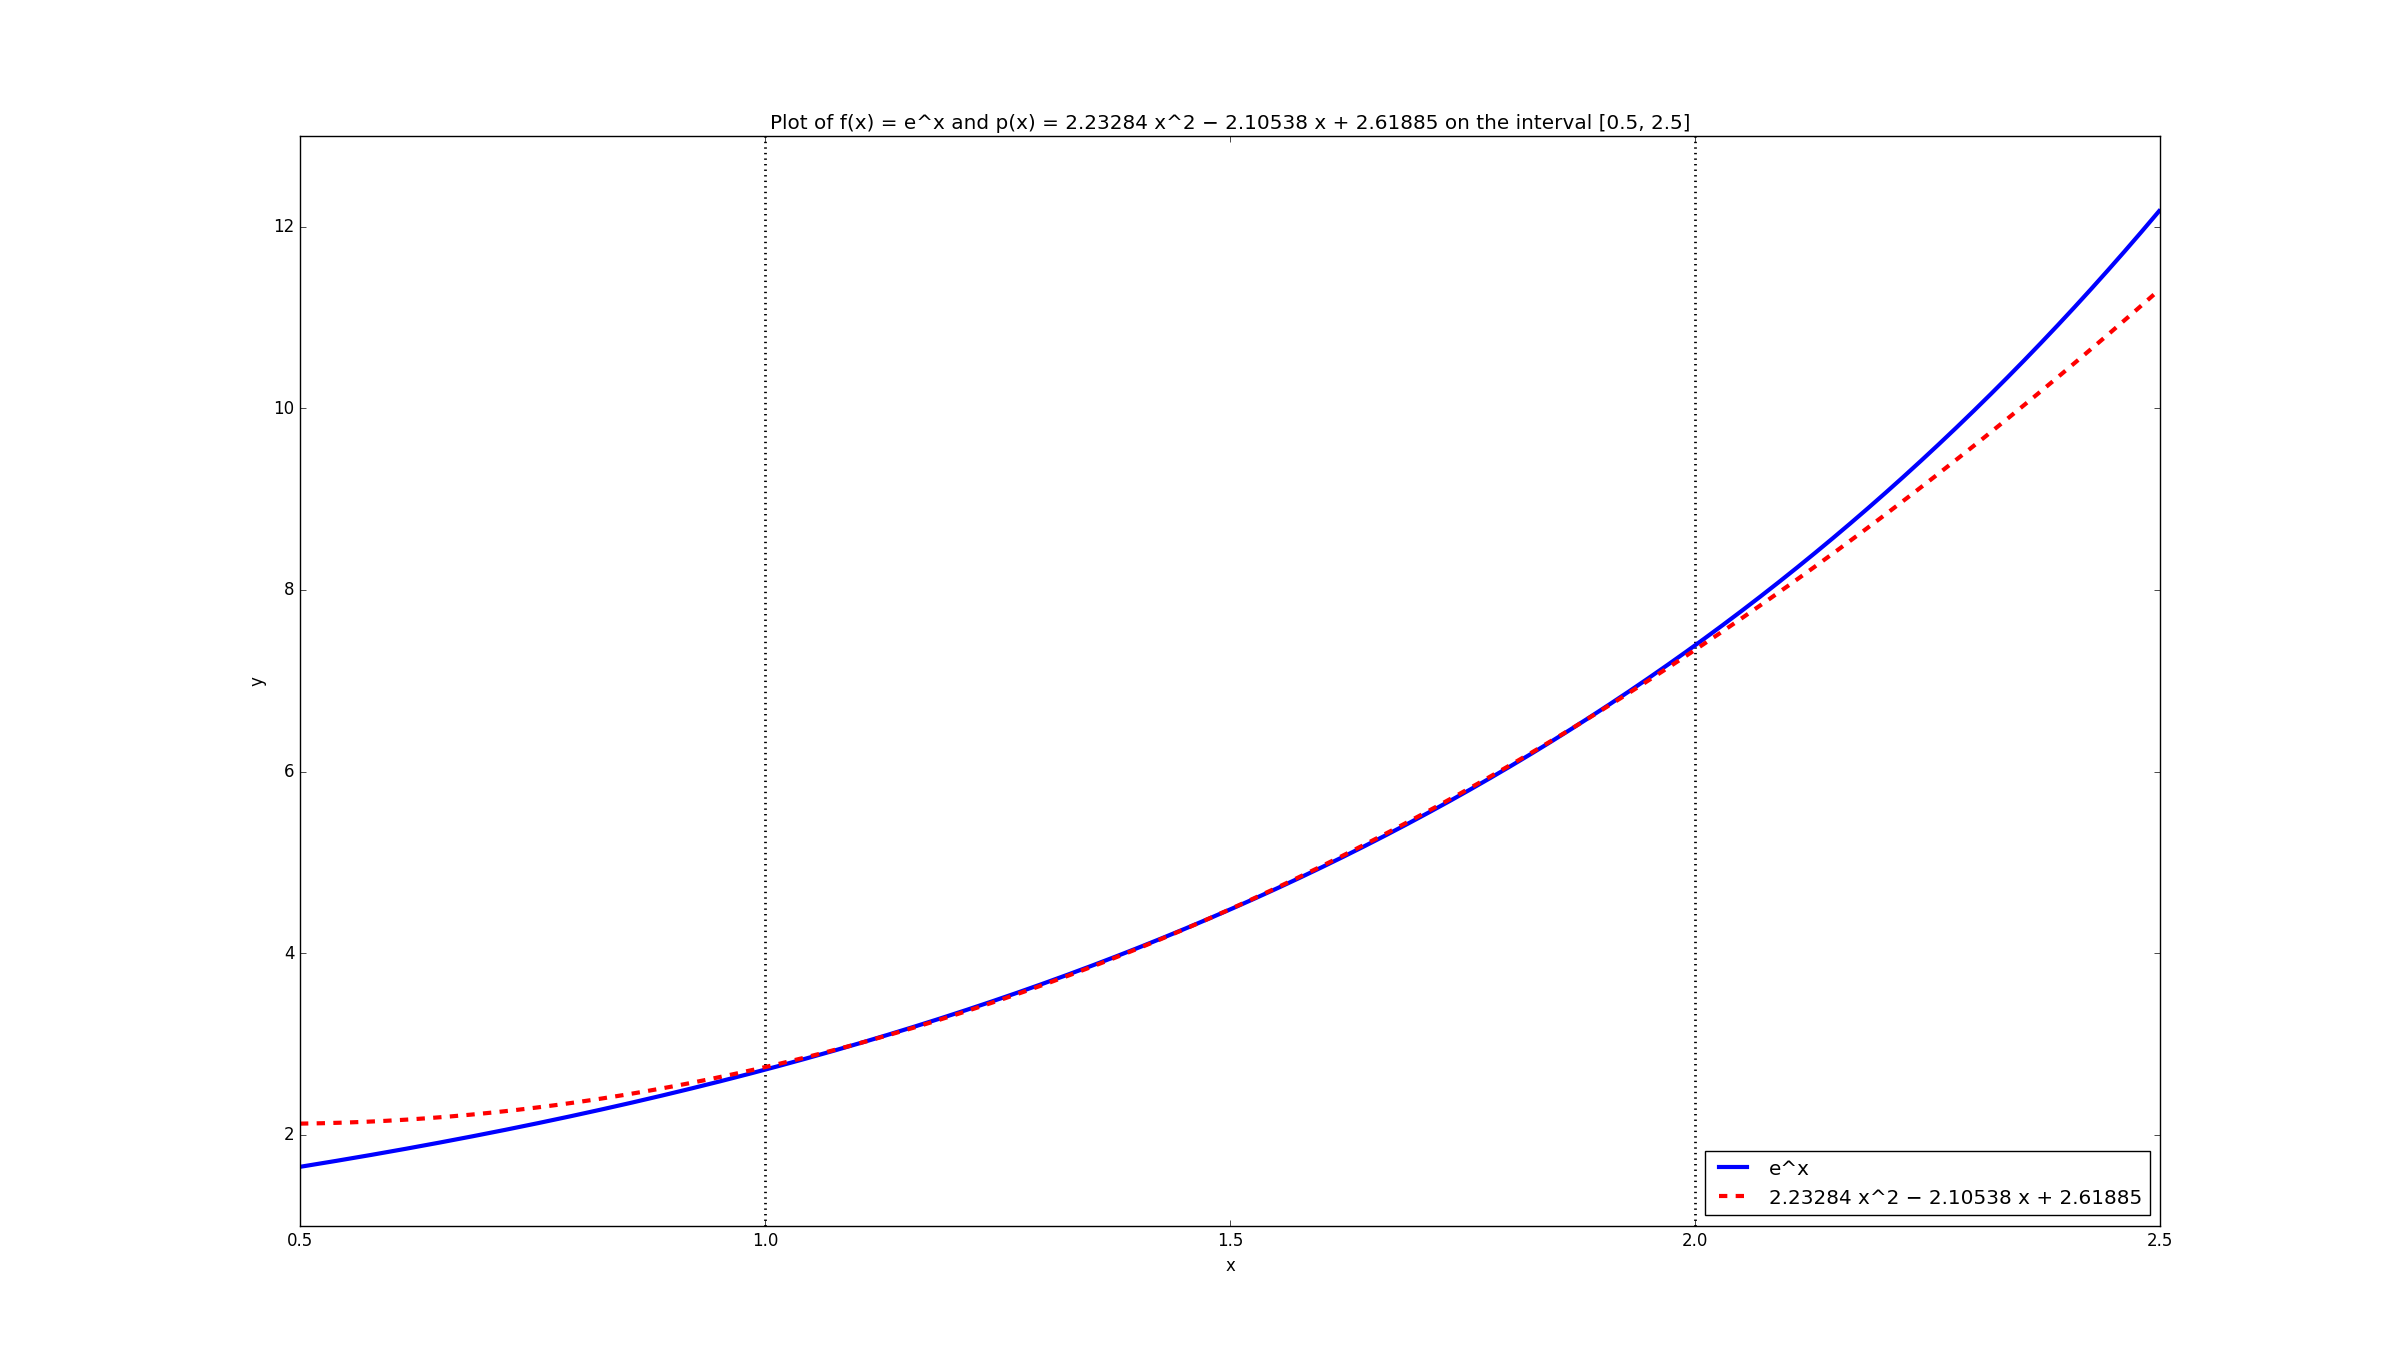
\includegraphics[trim={6cm, 0, 5cm, 2cm}, clip, width=\textwidth]{ortho_plot.png}
	\vspace{-10mm}
	\caption{Plot of $f(x) = e^x$ (solid line) and $p(x) = 2.23284 x^2 - 2.10538 x + 2.61885$ (dashed line), the polynomial constructed in 2 (a).}
	\label{Figure 1}
\end{figure}

% Stuff for wolfram alpha to simplify
(\frac{1}{4} n^2 + \frac{1}{4} n) (\frac{5}{4} n^2 + \frac{13}{4} n + \varepsilon) - n (\frac{5}{12} n^3 + \frac{9}{8} n^2 + \frac{17}{24} n + \delta)

(\frac{1}{4} n^2 + \frac{1}{4} n)^2 - n (\frac{1}{12} n^3 + \frac{1}{8} n^2 + \frac{1}{24} n)

% Incorrect work for #3
Hence $$\phi_0 (t) = \sqrt{1/2}, \ \ \ \phi_1 (t) = \sqrt{3/2} \ (t + 2), \ \ \ \text{and} \ \ \ \phi_2 (t) = \sqrt{5/8} \ (3t^2 + 12 t + 11).$$ Now by defining $f(t) = e^{t + 2}$ we have $$p_2 (t) = \langle f(t), \phi_0 \rangle \phi_0 + \langle f(t), \phi_1 \rangle \phi_1 + \langle f(t), \phi_2 \rangle \phi_2.$$ Since $$\langle f(t), \phi_0 \rangle = e^2 \sqrt{\frac{1}{2}} \int_{-1}^{1} e^t \approx 12.28050385,$$ $$\langle f(t), \phi_1 \rangle = e^2 \sqrt{\frac{3}{2}} \int_{-1}^{1} e^t (t + 2) = 2 e^3 \sqrt{\frac{3}{2}} \approx 49.19931667,$$ and $$\langle f(t), \phi_2 \rangle = e^2 \sqrt{\frac{5}{8}} \int_{-1}^{1} e^t (3t^2 + 12t + 11) = e^2 \left( 14 e - \frac{2}{e} \right) \sqrt{\frac{5}{8}} \approx 218.0081755$$ we have that 
\begin{align*}
p_2 (t) = 12.28050385 \sqrt{\frac{1}{2}} + 49.19931667 (t + 2) \sqrt{\frac{3}{2}} + 218.0081755 (3t^2 + 12 t + 11) \sqrt{\frac{5}{8}} \\
&= 
\end{align*}

% Some unused code
# Generate data set {(x_1, y_1), ..., (x_20, y_20)}
    for k in range(1, m + 1):
        # Initialize x_k = k/2
        x.append(k/2)

        # Initialize eps_k as a random number uniformly distributed in [-2, 2]
        epsilon = np.random.uniform(-2, 2)

        # Set y_k = 5x_k + 2 + eps_k
        y.append(5*k/2 + 2 + epsilon)
